% --------------------------------------------------------------
% This is all preamble stuff that you don't have to worry about.
% Head down to where it says "Start here"
% --------------------------------------------------------------
 
\documentclass[12pt]{article}
 
\usepackage[margin=1in]{geometry} 
\usepackage{amsmath,amsthm,amssymb}
\usepackage{graphicx}
\newcommand{\N}{\mathbb{N}}
\newcommand{\Z}{\mathbb{Z}}
 
\newenvironment{theorem}[2][Theorem]{\begin{trivlist}
\item[\hskip \labelsep {\bfseries #1}\hskip \labelsep {\bfseries #2.}]}{\end{trivlist}}
\newenvironment{lemma}[2][Lemma]{\begin{trivlist}
\item[\hskip \labelsep {\bfseries #1}\hskip \labelsep {\bfseries #2.}]}{\end{trivlist}}
\newenvironment{exercise}[2][Exercise]{\begin{trivlist}
\item[\hskip \labelsep {\bfseries #1}\hskip \labelsep {\bfseries #2.}]}{\end{trivlist}}
\newenvironment{reflection}[2][Reflection]{\begin{trivlist}
\item[\hskip \labelsep {\bfseries #1}\hskip \labelsep {\bfseries #2.}]}{\end{trivlist}}
\newenvironment{proposition}[2][Proposition]{\begin{trivlist}
\item[\hskip \labelsep {\bfseries #1}\hskip \labelsep {\bfseries #2.}]}{\end{trivlist}}
\newenvironment{corollary}[2][Corollary]{\begin{trivlist}                      
\item[\hskip \labelsep {\bfseries #1}\hskip \labelsep {\bfseries #2.}]}{\end{trivlist}}
\newenvironment{definition}[2][definition]{\begin{trivlist}                      
\item[\hskip \labelsep {\bfseries #1}\hskip \labelsep {\bfseries #2.}]}{\end{trivlist}}
 
\begin{document}
 
% --------------------------------------------------------------
%                         Start here
% --------------------------------------------------------------
 
%\renewcommand{\qedsymbol}{\filledbox}
 
\title{Homework \#5}%replace X with the appropriate number
\author{\\ %replace with your name
CPSC 395 - Analysis of Algorithms
\\ Due: Monday, 15} %if necessary, replace with your course title
\date{}
\maketitle

\begin{enumerate}
\item Exercise 8.1-3 \\
Show that there is no comparison sort whose running time is linear for at least half of the n! inputs of length n. What about a fraction of 1/n of the inputs of length n? What about a fraction $1/2^n$? \\

From Theorem 8.1, with a tree of height h and l reachable leaves corresponding to a comparison sort on n elements we get n! $\leq$ l $\leq$ $2^h$. So we will use the same argument for the following. \\

For half of the input of length n, we have n!/2 $\leq$ n! $\leq$ l $\leq$ $2^h$. Again by going by Theorem 8.1, we will take the logarithms and we end up with h $\geq$ lg(n!/2). lg(n!/2) is equal to lg(n!) - lg(2) due to logarithmic identities. lg(n!) - lg(2) can be made into lg(n!) - 1, since lg is base 2. From Theorem 8.1, we can see that we would get $\Omega$(nlgn) - 1 or just $\Omega$(nlgn). So we can see it isn't linear.\\

For 1/n of the input of length n, we have (1/n)n! $\leq$ n! $\leq$ l $\leq$ $2^h$. We will take the logarithms and get h $\geq$ lg(n!/n). Again from logarithm identities, we will get lg(n!) - lg(n). We are able to do $\Omega$(nlgn) - lg(n), which we will again see isn't linear.\\

For $1/2^n$ of the input of length n, we have (1/$2^n$)n! $\leq$ n! $\leq$ l $\leq$ $2^h$. We will take the logarithms and get h $\geq$ lg(n!/$2^n$) which can also be written as lg(n!) - lg($2^n$). We will be able to get $\Omega$(nlgn) - n. We get the n since the base and argument are equal. We see that this isn't linear either. \\ 

\item Exercise 8.2-2 (The proof is just an explanation of why it is stable.) \\
Prove that COUNTING-SORT is stable. \\
When an algorithm is stable, that means numbers with the same value appear in the output array in the same order as they do in the input array. This means in an example array of [1,5,7,1] the 1 in the first position of the array and before the 1 in position 4, after the sorting in the final array the 1 from the first position will stay in the first position and be in front of the second 1 that will then be in the second position.

\item Exercise 8.3-1 \\
Using Figure 8.3 as a model, illustrate the operation of RADIX-SORT on the following list of English words: COW, DOG, SEA, RUG, ROW, MOB, BOX, TAB, BAR, EAR, TAR, DIG, BIG, TEA, NOW, FOX.\\
This is figure 8.3 as the model.\\
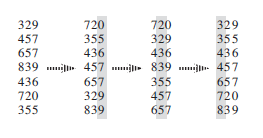
\includegraphics[scale=1]{radix.png} \\
The first set of columns is the initial list, the second set is the sorting by the value in the right column, the third set is the sorting by the value in the middle column, and the fourth set is the final sorting by the value in the left column. Now we do the same thing with the list of words but sorting it alphabetically. Also for radix sort to work correctly, it must be stable.\\
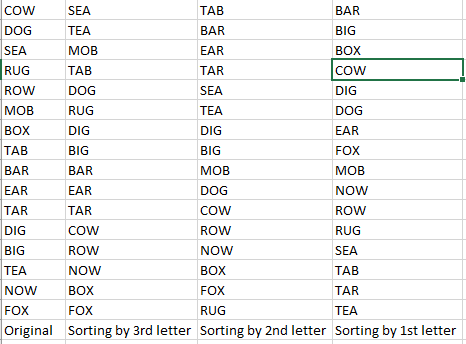
\includegraphics[scale=1]{Radix2.png}

\item Implement Counting-Sort (page 195) as function in Colab. The input should be $A$ and $k$ only. Your function should return $B$, the sorted array. The public link to your code should be in the body of your email.

\end{enumerate}
 
 
 Please email me if you have any questions.

% --------------------------------------------------------------
%     You don't have to mess with anything below this line.
% --------------------------------------------------------------
 
\end{document}